\documentclass[conference]{IEEEtran}
\IEEEoverridecommandlockouts
\usepackage{graphicx}
\usepackage{svg}
\usepackage{amsmath,amssymb,amsfonts}
\usepackage[natbib=true, style=numeric, sorting=none]{biblatex}

\addbibresource{references.bib}

\begin{document}

\title{Satisfaction-modeling based on queuing duration and service interruptions}

\author{
    Hampus Avekvist \\
    \IEEEauthorblockA{
        \textit{Department of Engineering Sciences} \\
        \textit{University West}\\
        Trollhättan, Sweden \\
        hampus.avekvist@hey.com
    }
}

\maketitle

\begin{abstract}
    This article explores how queuing duration and service
    interruptions affect satisfaction from persons in a $M/M/c$
    queuing system \cite{ChukovaUcarQueuingSystems}. A simple model
    of satisfaction where queue duration and interruptions matter
    is proposed and a simulation using \verb|SimPy| \cite{SimPy}
    is performed. The results show that, as the number of services
    increase, so does the satisfaction. Though, the number of
    services don't meet the demand of the actors and and the
    general result is a low, yet increasing, satisfaction. The
    model is simple and therefore provides several limitations that
    could inspire further work.
\end{abstract}

\begin{IEEEkeywords}
    satisfaction modeling, service interruptions
\end{IEEEkeywords}

\section{Introduction}

Waiting in turn for something is a common human experience most
have experienced. Most, if not all, have been in a line at least
once, be it the grocery checkout line, college application or
just waiting your turn at the doctors'. Alongside waiting in line,
a part of the human experience is emotional and, for this work,
the change in satisfaction from waiting in a queue. The field
has previous work, originally developed by Agner Krarup Erlang
\cite{ErlangSandsynlighedsregning, NeuroLaunchMakingSomeoneWait}
in the early 1900s when Erlang aimed to figure out how many
operators were necessary for proper call handling in telephone
exchange systems.

The paper is divided into the following parts: Section
\ref{sec:method} that proposes a simplified model of simulating
satisfaction from actors in a system based on the $M/M/c$
mathematical queuing model \cite{ChukovaUcarQueuingSystems}.
Section \ref{sec:method} also provides details on how the
simulation is performed. \ref{sec:results} show the results
following the simulation and provides an analysis of the results
and then the paper concludes in section \ref{sec:conclusion}.

\section{Method}
\label{sec:method}

\subsection{The model}

The model is a satisfaction-oriented $M/M/c$
\cite{ChukovaUcarQueuingSystems} (see Fig.~\ref{fig:queue-diagram})
system with $c$ services, where actors start with a uniformly
distributed level of satisfaction in the range $[2, 5]$. There is
a secondary range, $[0, 5]$, for the current satisfaction of an
actor used for measurements in the simulation. The ranges are
arbitrarily chosen. $0$ is the lowest level of satisfaction and
will prompt an actor to leave the system. While the actor is in
the queue, the satisfaction will decrement, alongside if they
face any difficulties using a service. 

\begin{figure}[!t]
    \centerline{
        \includesvg[width=0.25\textwidth]{figures/queue-model.svg}
    }
    \caption{
       A visual representation of what the queue can look like.
       Circles are actors, while the boxes at the top are service
       desks.
    }
    \label{fig:queue-diagram}
\end{figure}

Actors join the queue with an arrival rate of $13$ actors per $60$
minutes. If an actor faces difficulties using the service, an
arbitrary extra 30 seconds is added to the simulation time and
the actor retries. The actor retries until either the level of
satisfaction drops to $0$ or until they have finished using the
service. If an actor has been in the queue for at least $10$
minutes, they will lose one level of satisfaction and this repeats
until they either enter a service or satisfaction reaches $0$. The
actors utilize the service for a uniformly distributed simulated
time in the range $[0, 160]$ minutes. The following equation
\ref{eq:service-rate} gives the service rate where $S$ denotes the
service rate and $c$, as above, denotes the number of services.
$80$ is the average utilization time from the previously stated
range. 

\begin{equation}
    S(c) = \frac{c}{80}
    \label{eq:service-rate}
\end{equation}

\subsubsection{Limitations}

The following limitations provide possible ideas for further work.

\begin{itemize}
    \item The model is limited to an unoccupied queue
        \cite{NeuroLaunchMakingSomeoneWait}.
    \item The model doesn't allow people to know how long they
        will be standing in line \cite{NeuroLaunchMakingSomeoneWait}.
    \item The model assumes no cultural bias
        \cite{NeuroLaunchMakingSomeoneWait}.
    \item The model is a serpentine and not a parallel queue
        \cite{NeuroLaunchMakingSomeoneWait}.
    \item Not based on real data. Data from real experiments with
        similar scenarios are required.
    \item The model only accounts for satisfaction. A person
        could e.g. be more or less patient which may affect total
        satisfaction but won't be factored in this model.
    \item The queue requires active participation to remain in
        place and is not a ``sign-up and be notified'' type of
        queue that would allow simultaneous activity.
    \item The queue is ``perpetual'' and people can come and go
        as they like. A realistic situation would be a queue tied
        to working hours that could affect customer satisfaction
        from no longer accepting requests past a certain time.
\end{itemize}

\subsection{The simulation}

The simulation software Phone Service from
\cite{AvekvistLorentzonDta400}, based on \verb|SimPy| \cite{SimPy},
codifies the model above with applied values. The number of actors
in the system is hard-coded to $800$, arbitrarily chosen, alongside
a constant arrival rate at $13$ actors joining the system per $60$
minutes. The simulation generates data that is saved in a
\verb|SQLite3| \cite{SQLite3} database file that a secondary
program in the same module, called \verb|database_reader.py|, uses
to perform calculations and generate graphs. The simulation
software speaks in terms of phones and phone booths but the
simulation is more generalized so it may be used to simulate
general satisfaction-based systems where actors leave after
interruptions.

The data that is saved from the simulation is firstly the
satisfaction at the start of the simulation for every actor, paired
with the number of services available for the simulation
\cite{AvekvistLorentzonDta400}. Secondly, the service- and arrival
rates are stored and lastly the end result of the simulation is
saved. The end results contain the queue size upon an actor's
arrival in the queue, the queue duration and satisfaction for said
actor, alongside the number of services for this simulation. The
data is used by \verb|database_reader.py| to calculate averages and
generate the graphs provided in section \ref{sec:results}.

\section{Results}
\label{sec:results}

The results are provided from running the simulations $10$ times
for each $c$ and $\forall c \in [1, 100], c \in \mathbb{N}$. This
is to reduce the bias from the random number generator.

Firstly, as the number of services increase linearly, so does the
service rate. This follows from (\ref{eq:service-rate}) and is
shown in Fig.~\ref{fig:service-rate}. Furthermore, the queue time
is reduced in a linear-looking manner shown by
Fig.~\ref{fig:queue-time}. Lastly, the satisfaction increases
linear-like as shown in Fig.~\ref{fig:satisfaction}.

\begin{figure}[!b]
    \centerline{
        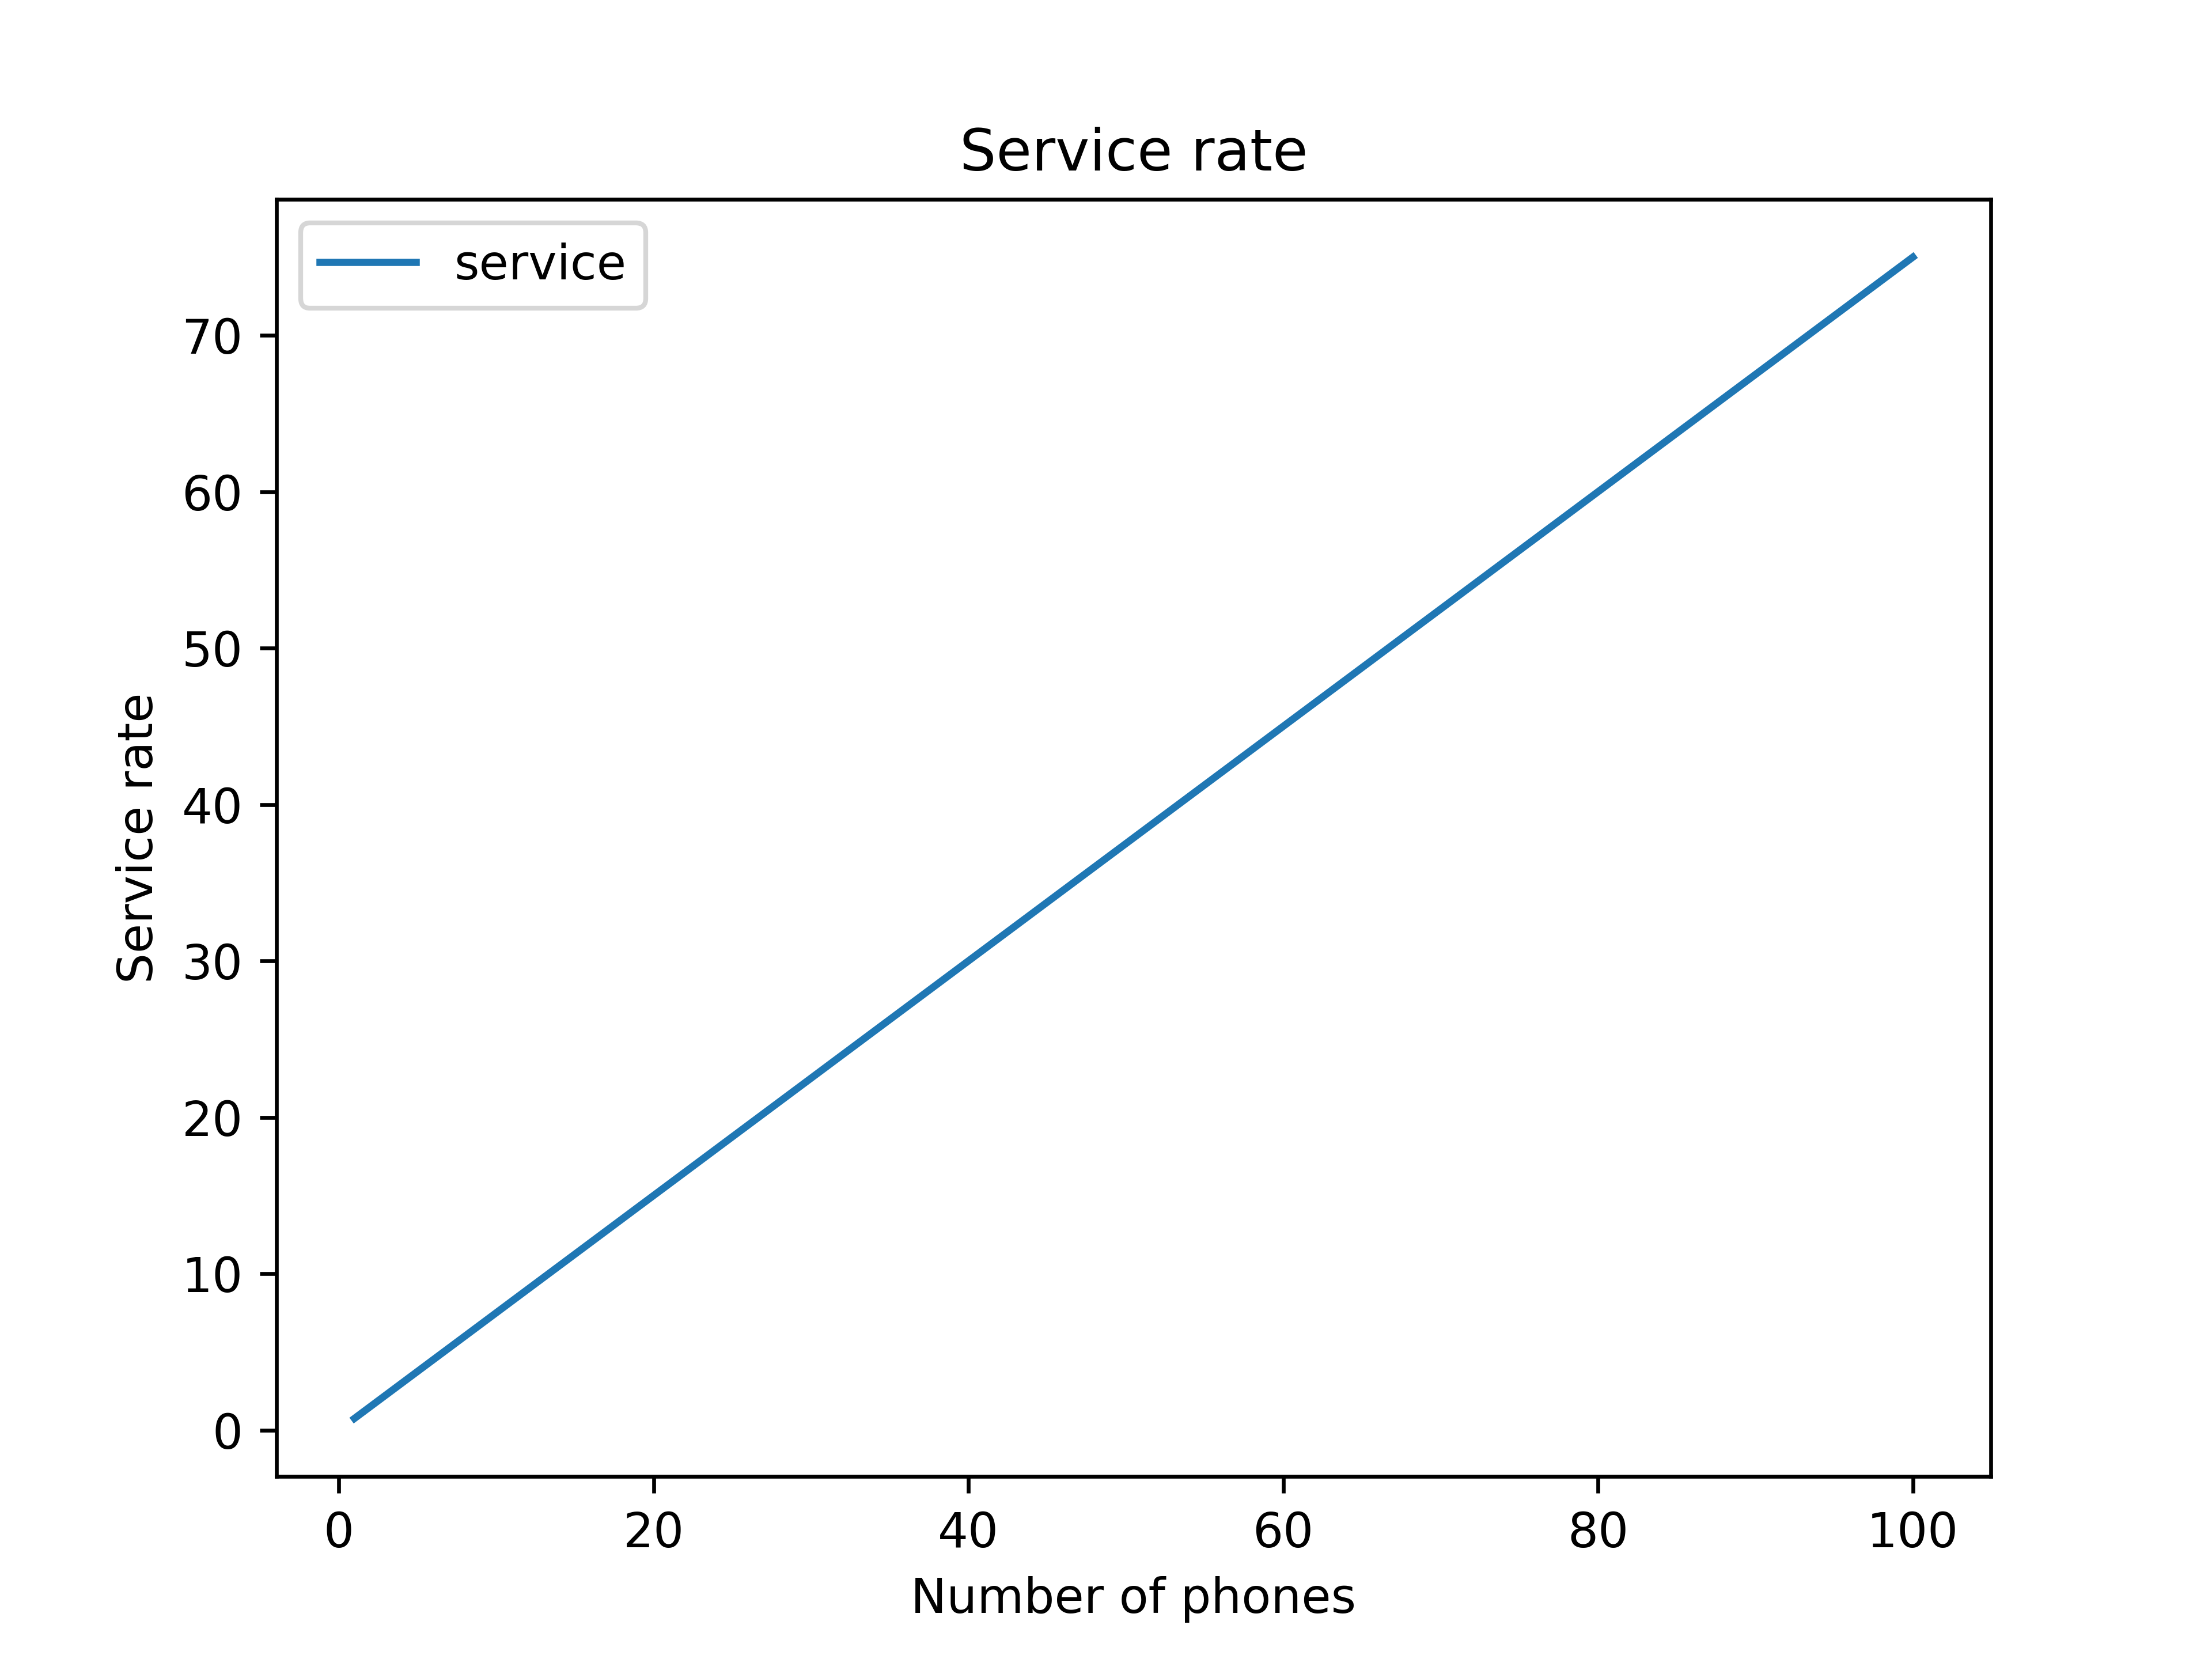
\includegraphics[width=0.4\textwidth]{figures/service.png}
    }
    \caption{
        The service rate linearly increases as the number of 
        services (phones) do, based on (\ref{eq:service-rate}).
    }
    \label{fig:service-rate}
\end{figure}

\begin{figure}[!t]
    \centerline{
        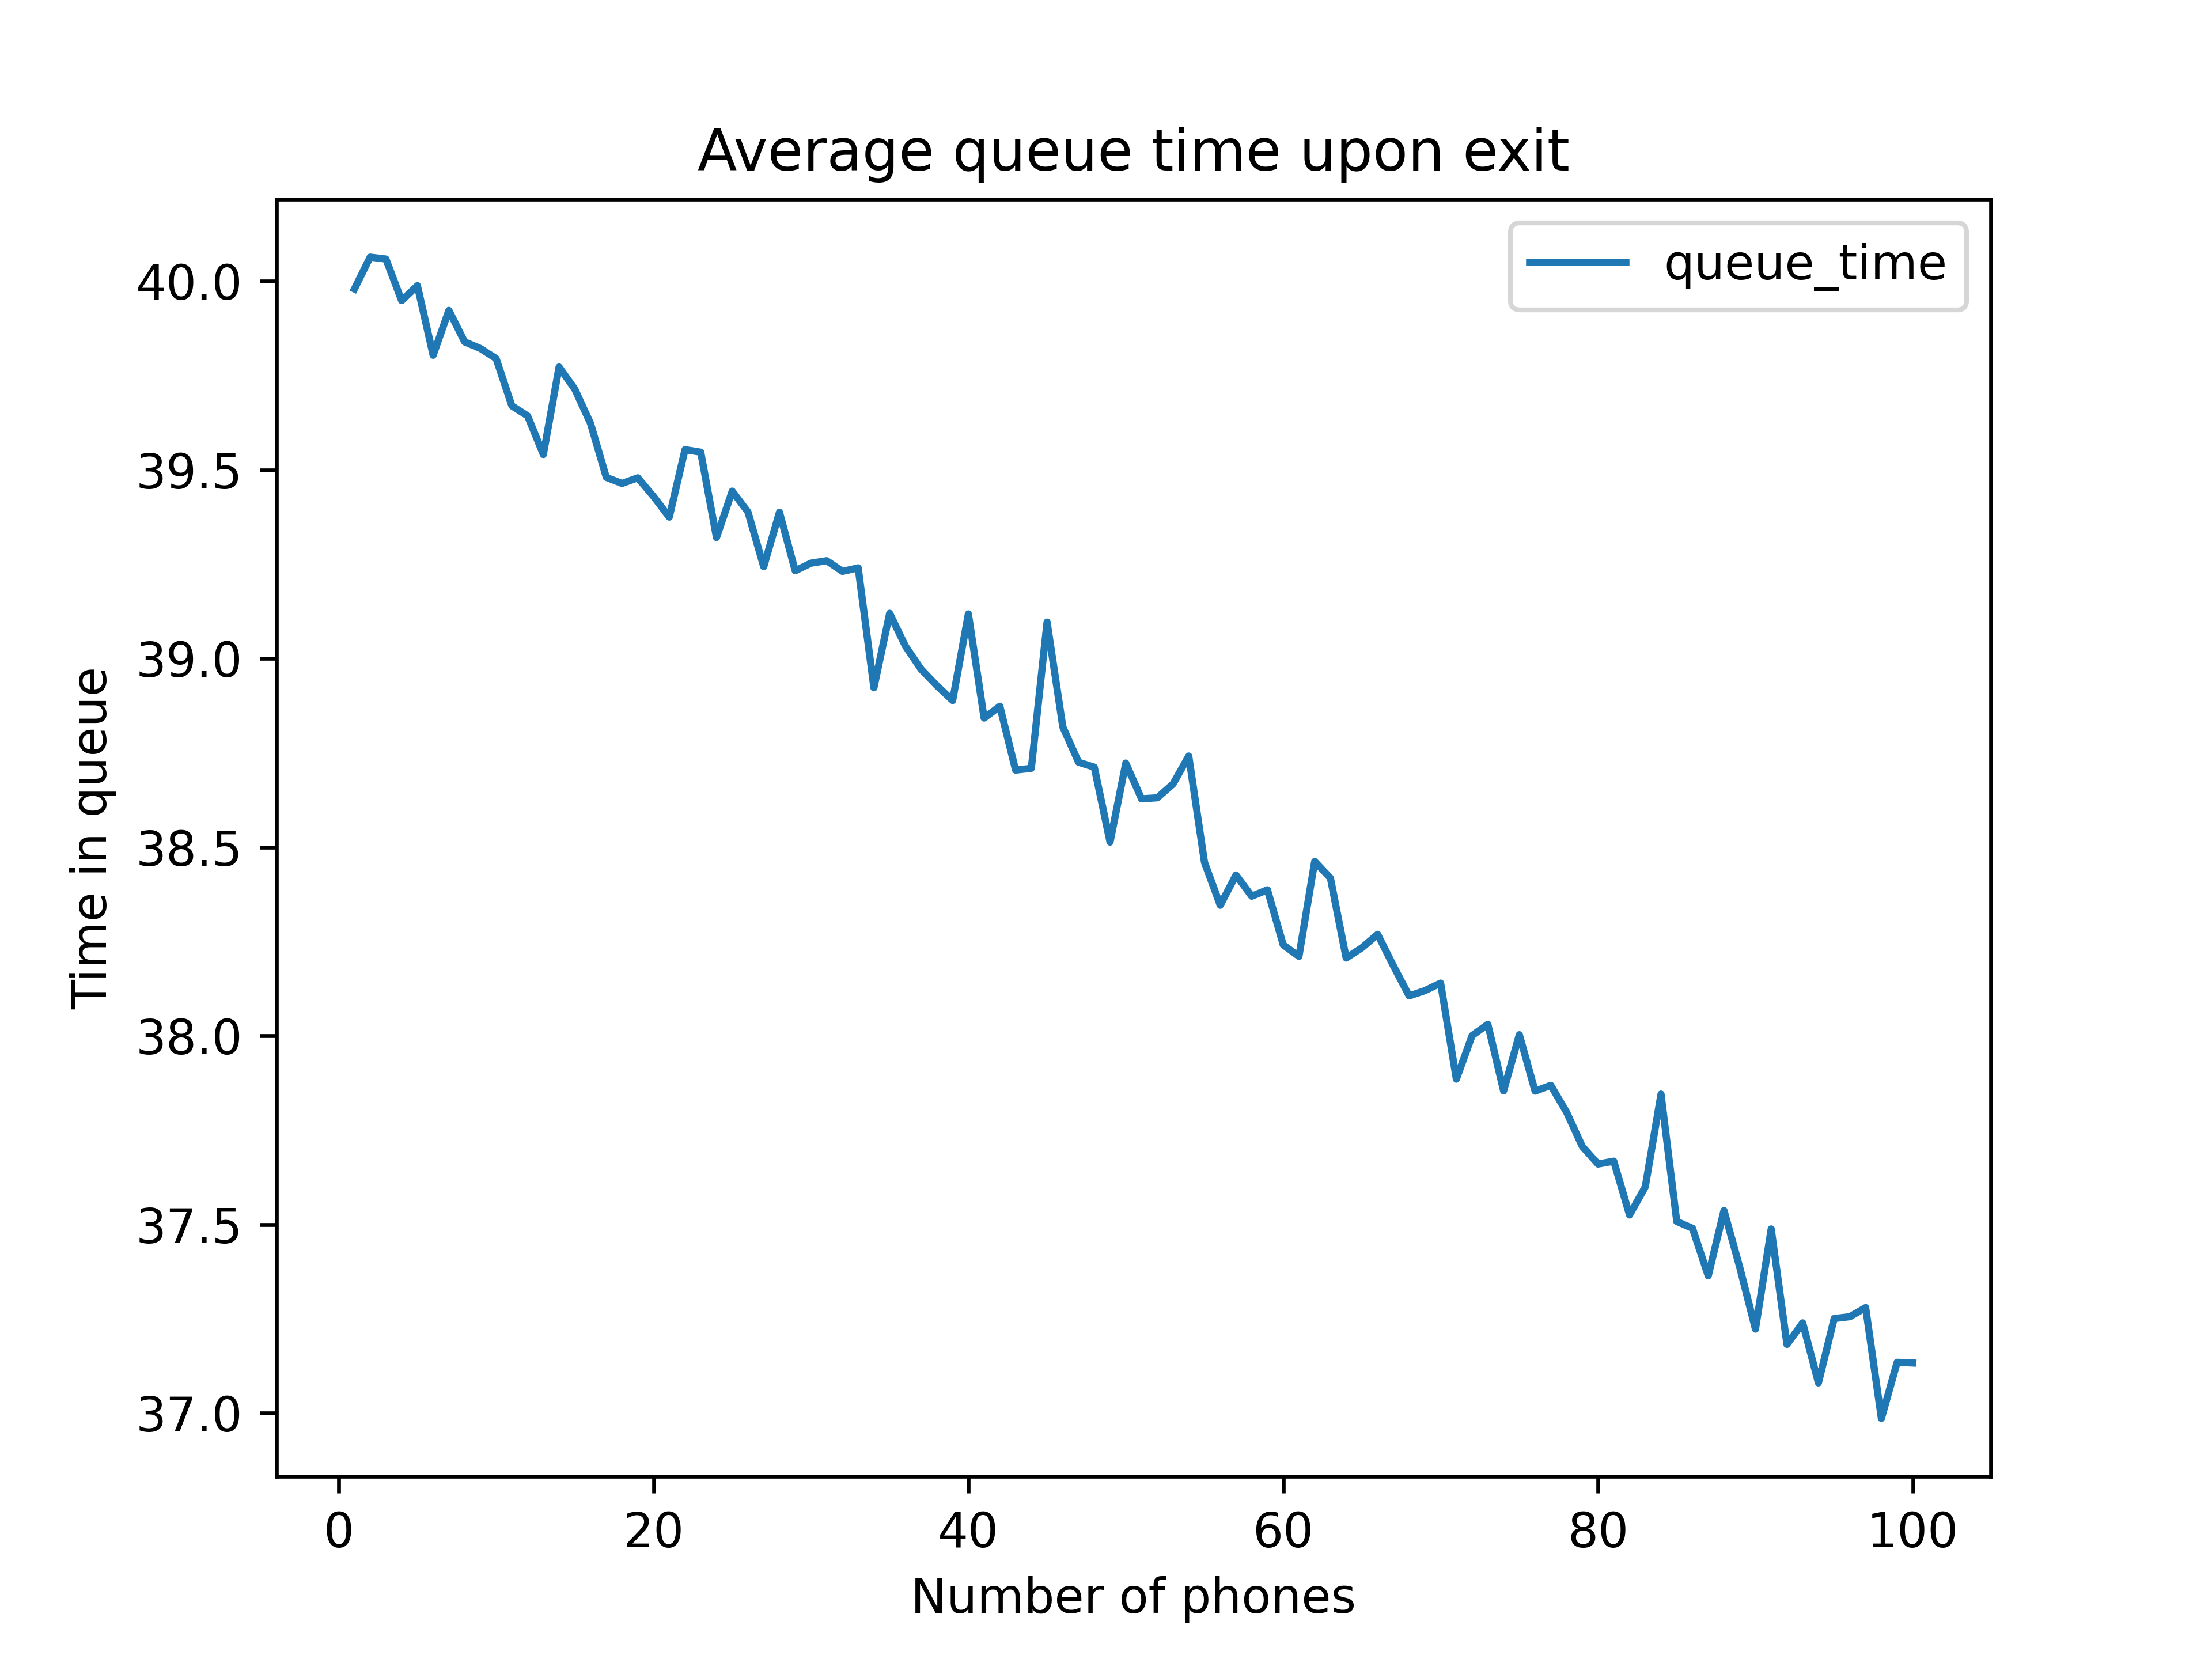
\includegraphics[width=0.4\textwidth]{figures/queue_time.png}
    }
    \caption{
        The average time an actor was in the queue decreases as
        the number of phones (services) do.
    }
    \label{fig:queue-time}
\end{figure}

\begin{figure}[!b]
    \centerline{
        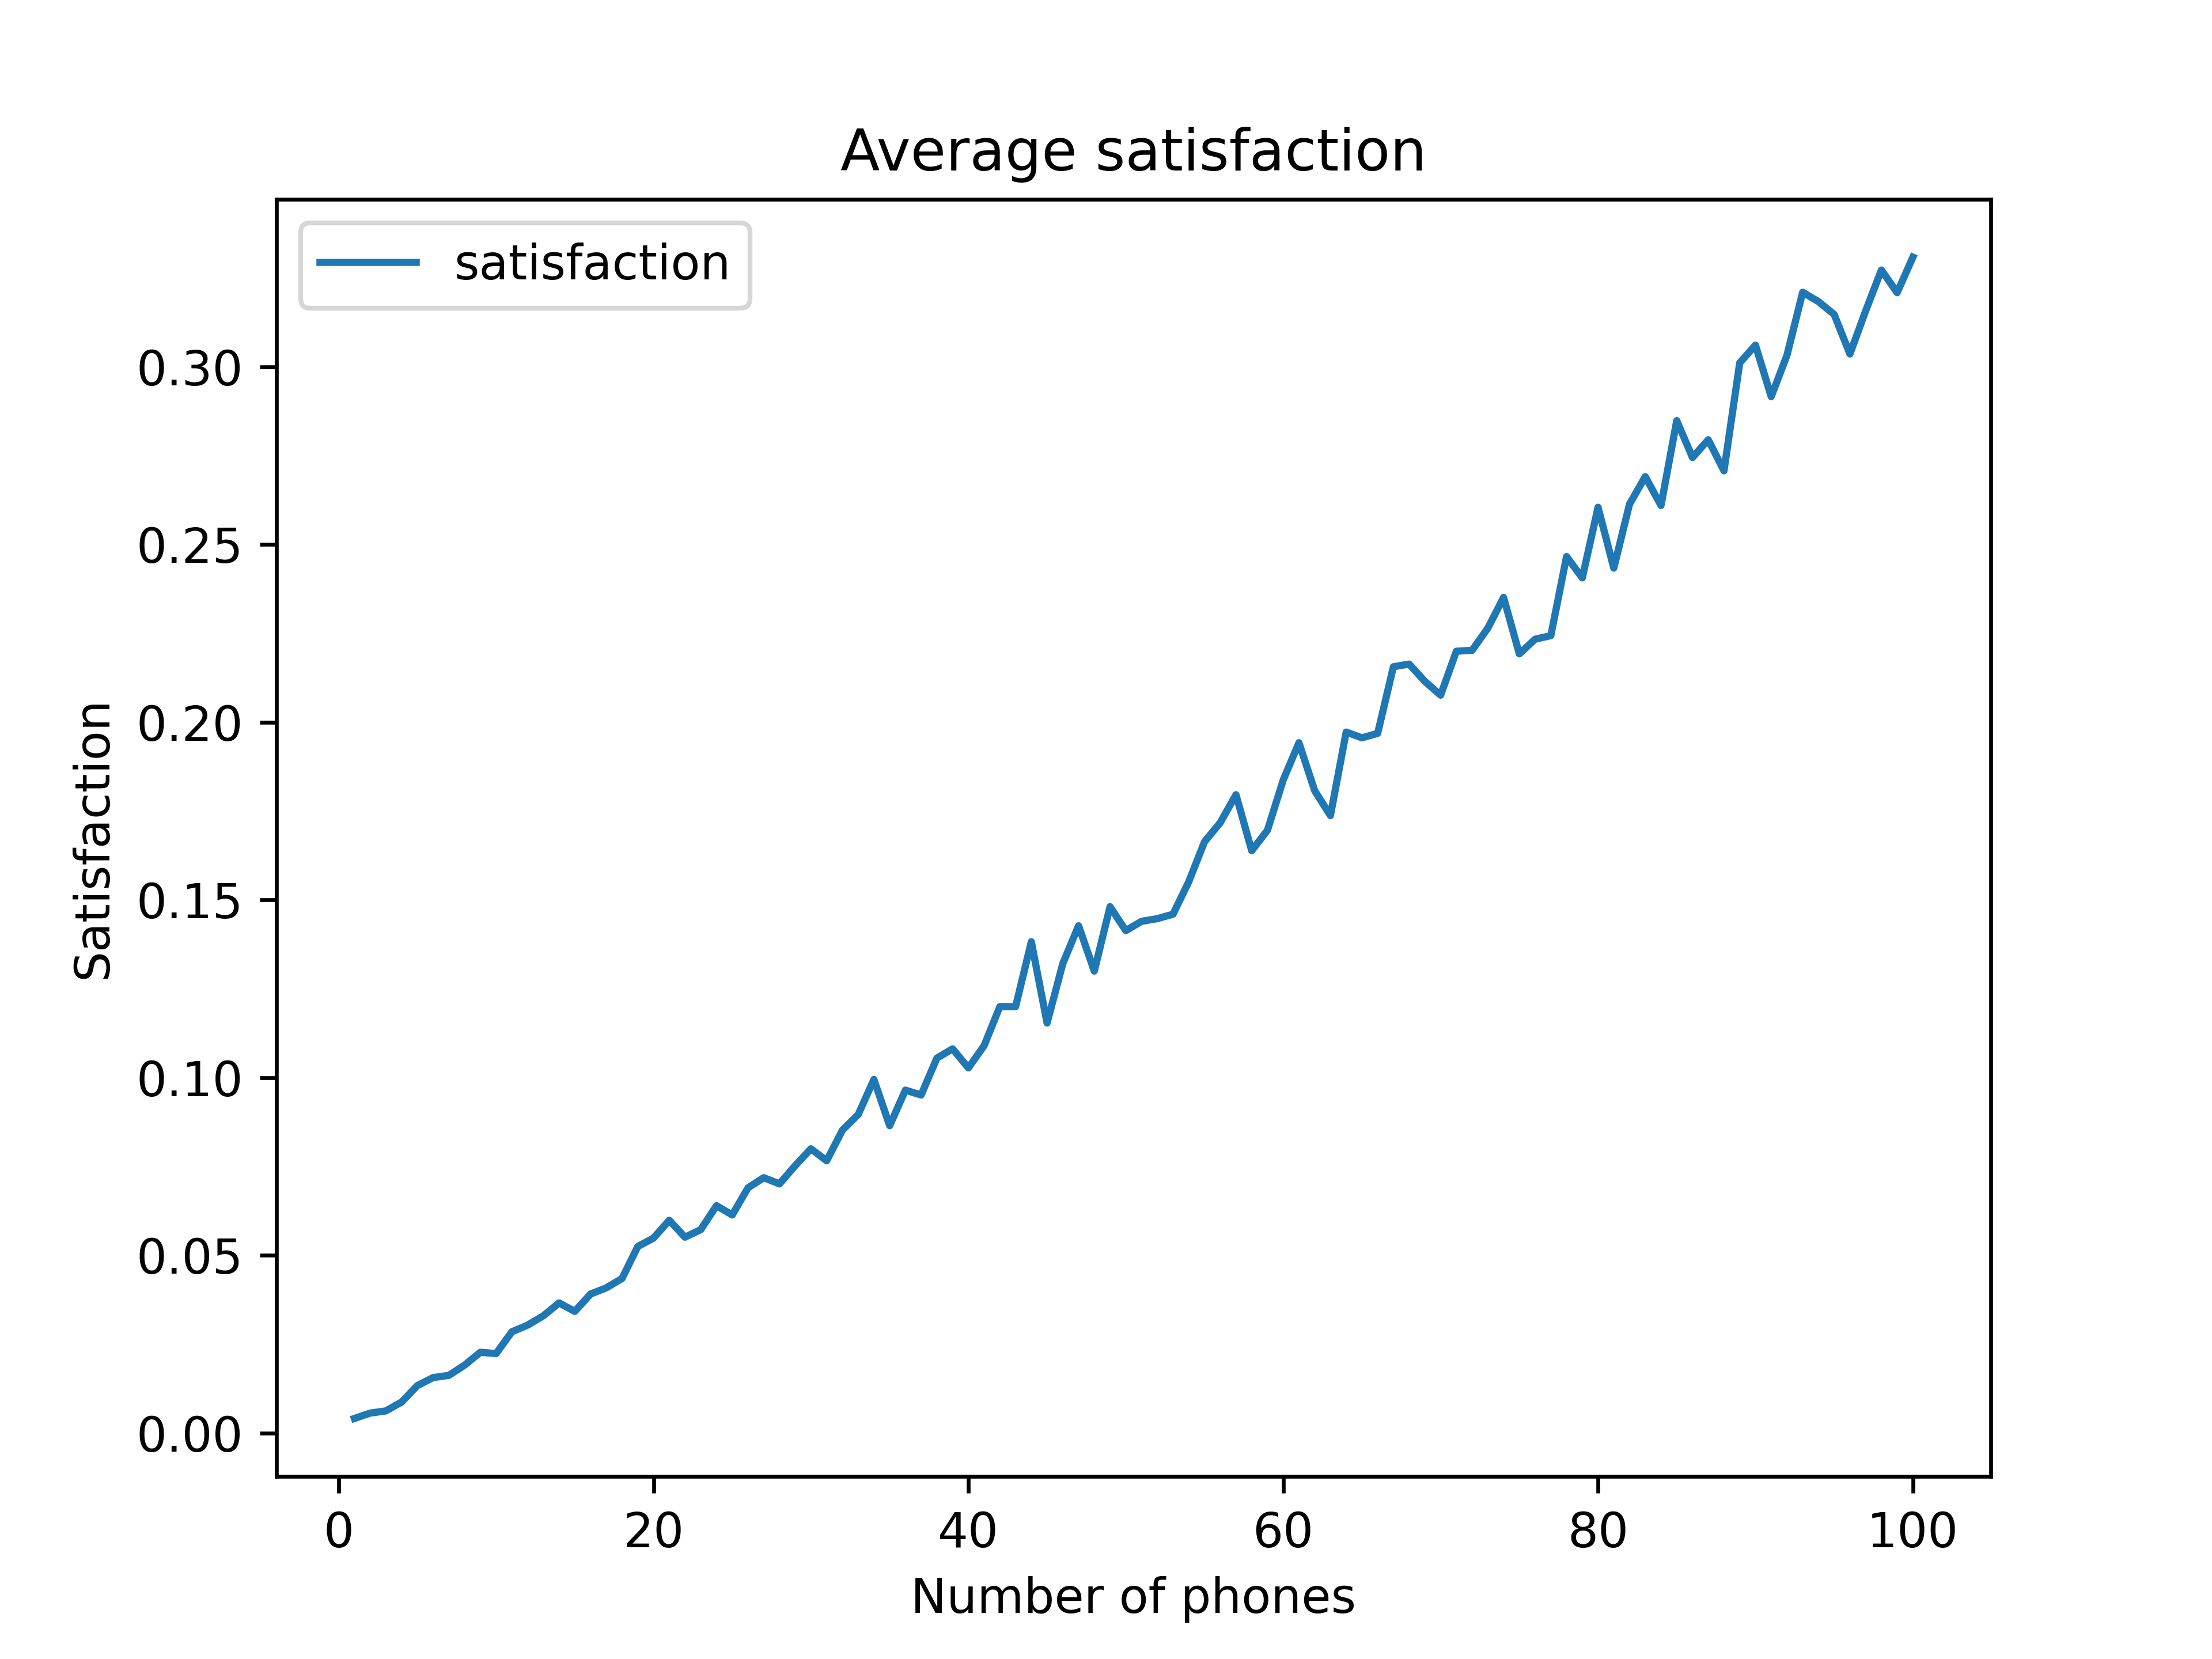
\includegraphics[width=0.4\textwidth]{figures/satisfaction.png}
    }
    \caption{
        The average satisfaction increases as the number of
        phones (services) do.
    }
    \label{fig:satisfaction}
\end{figure}

As the number of services increase, so does the satisfaction. This
is not unexpected, as more actors can be served at the same time,
which also decreases the time in line. Though, as
Fig.~\ref{fig:satisfaction} shows, most actors are either entirely
dissatisfied ($0$), or very dissatisfied, on the brink of leaving
the system. This is shown by Fig.~\ref{fig:queue-time} as actors,
on average, remain in the system between $37$ and $40$ minutes.
Since an actor loses a level of satisfaction per $10$ minutes spent
in queue, they lose $3$ to $4$ levels of satisfaction simply by
remaining in line. The starting level of satisfaction is uniformly
distributed in the range of $[2, 5]$, meaning a majority of actors
will leave the system. Though, as actors leave the system, other
actors reduce their waiting time, leading to the spikes in the 
graph.

\section{Conclusion}
\label{sec:conclusion}

The satisfaction increases as the queue time is reduced, which
depends on how many services that are available in the system.

\newpage

\section*{Acknowledgment}
\label{sec:acknowledgment}

I'd like to thank Felicia Lorentzon for the assistance and ideas
when working on the simulation, as well as the zany jokes we've
made along the way to keep us sane during the long hours. I'd also
like to thank Rashid Ali for his assistance when we had questions
and problems with our simulation and when we wanted to change our
model.

\printbibliography

\end{document}
